\documentclass[tikz,border=10pt]{standalone}
\usepackage[utf8]{inputenc}
\usepackage[T1]{fontenc}
\usepackage{amsmath}
\usepackage{helvet}
\usepackage{sansmath}
\renewcommand{\familydefault}{\sfdefault}
\usetikzlibrary{arrows.meta,calc,positioning}

% Paleta pastel
\definecolor{fBlue}{RGB}{232,241,252}   \definecolor{bBlue}{RGB}{140,176,216}
\definecolor{fGreen}{RGB}{232,246,236}  \definecolor{bGreen}{RGB}{140,196,160}
\definecolor{fRed}{RGB}{252,232,232}    \definecolor{bRed}{RGB}{226,140,140}
\definecolor{fGray}{RGB}{242,242,246}   \definecolor{bGray}{RGB}{170,170,182}
\definecolor{fYellow}{RGB}{252,248,224} \definecolor{bYellow}{RGB}{222,196,120}
\definecolor{txt}{RGB}{70,74,88}

\begin{document}
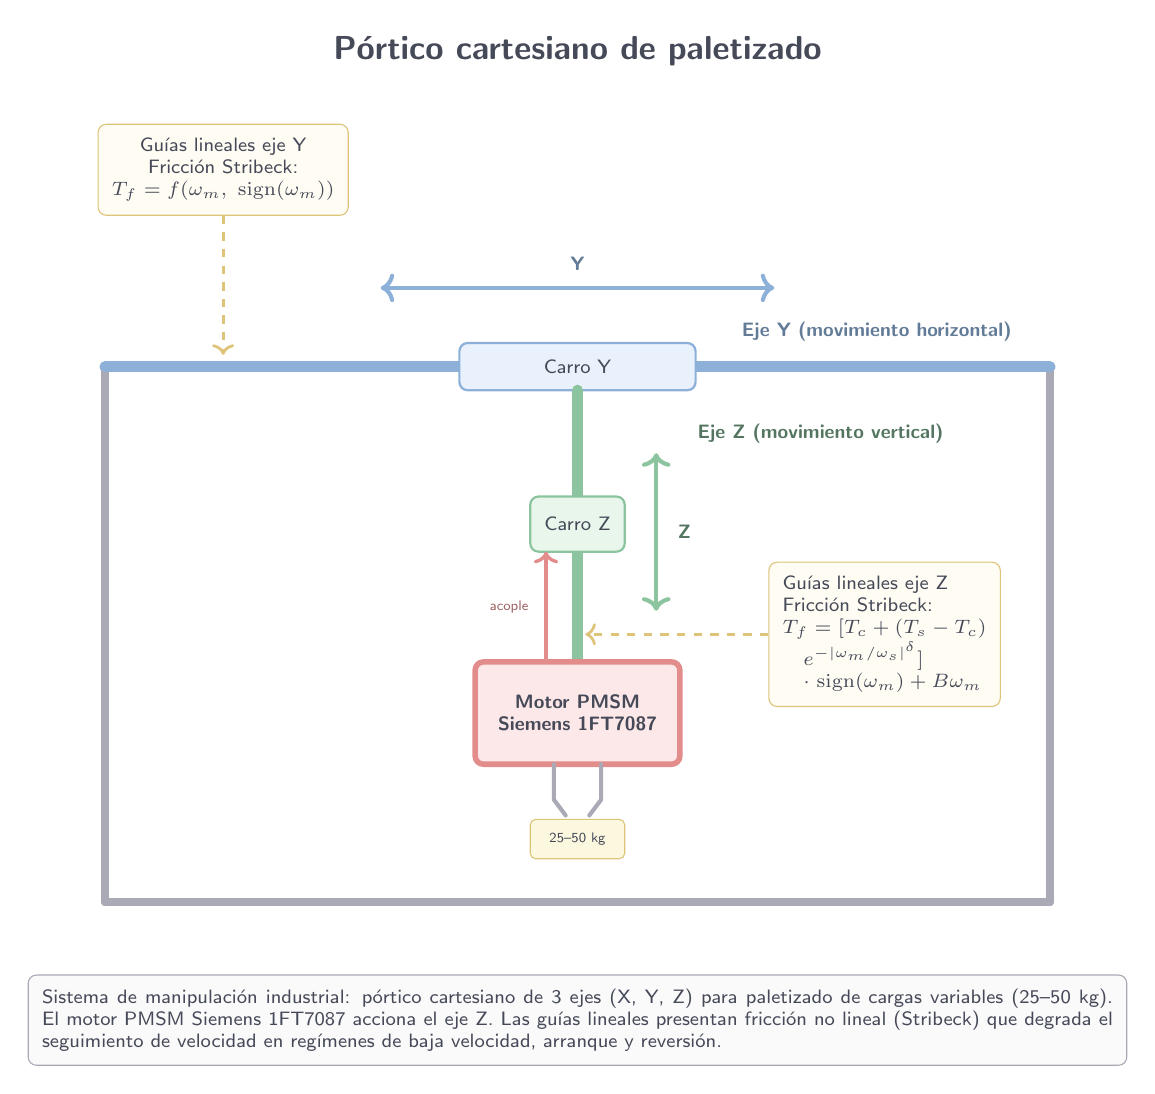
\begin{tikzpicture}[font=\scriptsize, text=txt]

% 1. Título
\node[font=\large\bfseries] at (7,10) {Pórtico cartesiano de paletizado};

% 2. Base (bajada a y=-0.8 para no pisar la caja de carga)
\draw[line width=3pt, bGray, line cap=round] (1,-0.8) -- (13,-0.8);

% 3. Columnas laterales
\draw[line width=3pt, bGray, line cap=round] (1,-0.8) -- (1,6);
\draw[line width=3pt, bGray, line cap=round] (13,-0.8) -- (13,6);

% 4. Viga superior (eje Y)
\draw[line width=4pt, bBlue, line cap=round] (1,6) -- (13,6);
\node[font=\scriptsize\bfseries, text=bBlue!70!black] at (10.8,6.45) {Eje Y (movimiento horizontal)};

% 5. Flecha eje Y
\draw[<->, line width=1.5pt, bBlue] (4.5,7.0) -- (9.5,7.0);
\node[font=\scriptsize\bfseries, text=bBlue!70!black] at (7,7.3) {Y};

% 6. Carro Y
\node[draw=bBlue, fill=fBlue, rounded corners=3pt, minimum width=3cm,
      minimum height=0.6cm, line width=0.8pt] (cy) at (7,6) {Carro Y};

% 7. Columna Z
\draw[line width=4pt, bGreen, line cap=round] (7,5.7) -- (7,2);
\node[font=\scriptsize\bfseries, text=bGreen!60!black, anchor=west] at (8.4,5.15) {Eje Z (movimiento vertical)};

% 8. Flecha eje Z
\draw[<->, line width=1.5pt, bGreen] (8.0,2.9) -- (8.0,4.9);
\node[font=\scriptsize\bfseries, text=bGreen!60!black, anchor=west] at (8.15,3.9) {Z};

% 9. Carro Z
\node[draw=bGreen, fill=fGreen, rounded corners=3pt, minimum width=1.2cm,
      minimum height=0.7cm, line width=0.8pt] (cz) at (7,4) {Carro Z};

% 10. Motor PMSM
\node[draw=bRed, fill=fRed, rounded corners=3pt, line width=2pt,
      minimum width=2.6cm, minimum height=1.3cm, align=center,
      font=\scriptsize\bfseries] (motor) at (7,1.6) {Motor PMSM\\Siemens 1FT7087};

% 11. Flecha de acople (desplazada a x=6.6 para no solaparse con la columna)
\draw[->, line width=1.2pt, bRed] (6.6,2.25) -- (6.6,3.65);
\node[font=\tiny, text=bRed!70!black, anchor=east] at (6.5,2.95) {acople};

% 12. Efector final
\draw[line width=1.5pt, bGray, line cap=round, line join=round]
  (6.7,0.95) -- (6.7,0.5) -- (6.85,0.3);
\draw[line width=1.5pt, bGray, line cap=round, line join=round]
  (7.3,0.95) -- (7.3,0.5) -- (7.15,0.3);
\node[draw=bYellow, fill=fYellow, rounded corners=2pt, minimum width=1.2cm,
      minimum height=0.5cm, font=\tiny] (caja) at (7,0) {25--50 kg};

% 13. Fricción guías eje Y
\node[draw=bYellow, fill=fYellow!40, rounded corners=3pt, align=center,
      font=\scriptsize, inner sep=5pt] (fy) at (2.5,8.5)
  {Guías lineales eje Y\\Fricción Stribeck:\\$T_f = f(\omega_m,\ \mathrm{sign}(\omega_m))$};
\draw[->, dashed, line width=1pt, bYellow] (fy.south) -- (2.5,6.15);

% 14. Fricción guías eje Z
\node[draw=bYellow, fill=fYellow!40, rounded corners=3pt, align=left,
      font=\scriptsize, inner sep=5pt] (fz) at (10.9,2.6)
  {Guías lineales eje Z\\Fricción Stribeck:\\
   $T_f = [T_c + (T_s - T_c)$\\
   $\quad e^{-|\omega_m/\omega_s|^{\delta}}]$\\
   $\quad \cdot\ \mathrm{sign}(\omega_m) + B\omega_m$};
\draw[->, dashed, line width=1pt, bYellow] (fz.west |- 7,2.6) -- (7.1,2.6);

% 15. Nota al pie
\node[draw=bGray, fill=fGray!40, rounded corners=3pt, text width=13.6cm,
      align=justify, font=\scriptsize, inner sep=5pt] at (7,-2.3)
  {Sistema de manipulación industrial: pórtico cartesiano de 3 ejes (X, Y, Z)
   para paletizado de cargas variables (25--50 kg). El motor PMSM Siemens
   1FT7087 acciona el eje Z. Las guías lineales presentan fricción no lineal
   (Stribeck) que degrada el seguimiento de velocidad en regímenes de baja
   velocidad, arranque y reversión.};

\end{tikzpicture}
\end{document}
